\chapter{\textbf{Mininet-WiFi Experiments}}
\label{chapter: Mininet-wifi Experiments}
This chapter describes the Mininet-WiFi experiment we conducted to validate the performance of our proposed user-manged edge-enabled SFC placement in practice. The MEC emulation is implemented as an extension to Mininet-WiFi\cite{mininetwifi}, Mininet-WiFi is a tool that allows researchers to emulate a wireless network environment using SDN technologies. It has supports for the wireless station, Access points, and mobility model. We started by describing the simulation setup and parameters in section \ref{sec:mininetwifisetup}. Then we present the results from the experiments we did in Mininet-WiFi including the learning behavior of \myalgorithm\ in Mininet-WiFi (section \ref{sec:mininetwifilearningbehavior}) and comparison with greedy algorithms under different environmental parameters (section \ref{sec:mobility model experiments}, \ref{sec:mininetwifinetworkdelays}, \ref{sec:mininetwifiSFClength}). 

% In this chapter, we conduct a series of Mininet-WiFi experiments to emulate the MEC wireless network and validate the performance of our SFC placement framework in practice. The MEC emulation is implemented as an extension to Mininet-WiFi\cite{mininetwifi}. Mininet-WiFi is a tool that allow researchers to emulate a wireless network environment using SDN technologies, it has supports for wireless station, Access points and mobility model etc. 



\section{Experiment setup.}
\label{sec:mininetwifisetup}
In our Mininet-WiFi emulation, we create an edge-enabled network with nine wireless base stations that are scattered in a $100\times100$ squared meter area, as shown in figure~\ref{fig:mininettopology}. Each base station is connected to a server that provides computation services. The user, who is connected to the closet base station automatically,  moves with a constant speed that is selected randomly from the interval [1, 5] meters per second. We use the log-distance propagation loss model for wireless connections. We use sockets that run on the edge servers to emulate the computation delay. The user repeatedly sends packets to the closest base station, where the packet is then forwarded to traverse the services in the chain. The last service in the chain sends a response back that allows the user service in the chain sends a response back that allows the user to collect the end-to-end delay (by time-stamping the packets).
The Mininet-WiFi environment is set up in a VM running Ubuntu 16.04.2 LTS with 2 cpu and 4GB RAM. The VM is deployed on a windows 10 machine with i5-7400 and 8GB of RAM.


%we simulate a MEC network that consist of 9 hosts, each of which are attached with an Access Point (AP) that can communicate with mobile user via WiFi and all host are connected using wired Ethernet connections. We then add a moving node as mobile user using a selected mobility model (with a maximum speed of 5 meters/second and minimum speed of 1 meter/s) and propagation model (The Log-Distance Propagation Model) that calculate the power of signal received by the mobile user.
%as show in figure \ref{fig:mininettopology}, the computing nodes are scattered in a 100x100m area with wireless signal range covered the entire area. The Mininet-WiFi environment is set up in a VM running Ubuntu 16.04.2 LTS with 2 cpu and 4GB RAM, which is hosted by a windows 10 machine (i5-7400 \& 8GB RAM).
\begin{figure}
	\centering
	\includegraphics[width=0.9\linewidth]{figs/mininetwifigraph.png}
	\vspace{\baselineskip}
	\caption{Mininet-WiFi Emulation}
	\label{fig:mininettopology}
\end{figure}
%On each edge node, we install server functions that listen for user's request and are configured with different values of computing latency. On user node, we install a client function that sends requests periodically to the servers with dynamic demands and listens for the response.

The parameters used in Mininet-WiFi simulation are summarized as follow:
\begin{itemize}
	\item \textbf{Duration} \textemdash Each experiments ran for 30-60 minutes 
	\item \textbf{Area} \textemdash the spatial area has a dimension $100 \times 100$ meters
	\item \textbf{Mobile stations} \textemdash there is one mobile station representing the mobile user with a mobility model
	\item \textbf{Packet generation rate} \textemdash 25-100 packets per time slot.
	\item \textbf{Packet size} \textemdash fixed to 1 byte.
	\item \textbf{Access Points} \textemdash 9 APs with fixed positions show in figure \ref{fig:mininettopology} with a connection range of 20 meters, which makes 99 \% of the simulation area covered by WiFi, with each of them connected to an edge server.
	\item \textbf{Mobility model} \textemdash five different mobility models analyzed in section \ref{sec:mobility model experiments}, with each configured with a maxmum speed of 5 meters/second and minimum speed of 1 meters/second.
	\item \textbf{Handover policies} \textemdash Active handover, a client station switches WiFi connections to an AP as soon as it finds another connection with closer range, this means that the client is always connected to the closet AP, which is the same as Networx simulation.
	\item \textbf{Propagation model} \textemdash The Log-Distance Propagation Model.
\end{itemize}
%The specifics of The Log-Distance Propagation Model are described as follow:
%
%
%Channel gain, $H$, is calculated by the path-loss with random shadowing,
%\begin{gather}
%    20\times \log{\{\text{distance}^{km}\}} + 28 + \mathcal{N}(0, 5^2), \\
%    H(t)=\frac{10^{-2.8}}{\text{distance}^{2}\times 10^{\mathcal{N}(0, 5^2)/10}}, \\
%    P=10^{1.5}mW.
%\end{gather}
%
%
%Power            = 15 dBm 
%noise            = normal(0,25)
%
%
%P  = 31.6 mW
%H  = 0.01
%Ii = 0.02 mW
%Im = 0.01 mW
%N  = N(0, 25) / 1000 mW
%
%Expect: 
%SNR (signal-to-noise ratio) = (HP)/(Ii+Im+N) = 10
%SNR = 0.316 / (0.03 + N)
%
%Allocated Bandwidth = 1Mhz
%
%Final Bandwidth = 3 Mbps


% \subsection{User machine settings}
% The user machine function as both the SFC request sender and the traffic generator. Specifically,
% the user first send the SFC placement request specifying the SFC placement and the last SFC placement, then a http request that includes all the contextual information above will be generated and sent to the first server on the SFC placement.
% Upon receiving the correct response, the user then start generating traffic and send it to the SFC. It then start listening for a response

% \subsection{Server settings}
% % In our experiment, we implement three VNFs includes an encoder, a decoder and a traffic monitor, which are implemented in Python.
% Accordingly,  the server is also consist of two parts: 
% \begin{enumerate}
%     \item A http server that receives and forwards the SFC placement request, it will also send a VNF migration request to its corresponding server in the last SFC placement; 
%     \item  After the migration and placement is done, the server then start a TCP server that listens for the traffic generated from user, when receiving the traffic, it process each packet with respect to a certain processing delay.
% \end{enumerate}
%  During a SFC placement, the user first sends a SFC placement & migration request, each server that received the request will start listening for traffic while forward the placement request to the next server, when the last server finish placement, it sends a response to user so the user can start sending traffic to the SFC.
%  An example of how the SFC is placed is shown in Figure \ref{fig:SFCplacementdiagramEmulation}, Particularly in Mininet-WiFi emulation, each access point function as both a wireless base station for user and a switch for edge server. 
% \begin{figure}
%     \centering
%     \includegraphics[width=0.9\linewidth]{figs/SFCtrafficmec.PNG}
%     \caption{A placemnent of a simple SFC in MEC}
%     \label{fig:SFCplacementdiagramEmulation}
% \end{figure}

% a TCP server that receives and forwards the traffic
% implemented by python Flask\cite{flask}. Specifically, when running the server, the operator can specify a processing delay, each server will the wait for a SFC request, upon receiving a request, each server will analyze the packet and extract the contextual information such as placement array, last placement array and demand, it first sends a switching request to corresponding server that runs the services in the last timeslot, it the delay the packet for the processing time specified and forward the request to the next placed node according to the placement array. 

% When the last server on the placement array finish its processing, it will return a packet to client.  Upon receiving the return packet, the client will stop recording the time and calculating a end-to-end delay.

% server code will be run on the server hosts

% \subsection{Estimation}
% % Besides SFC request, client can also send a estimation request to a specific computing node, when estimated node receive the request, it will evaluate its processing delay and return it to the client. Client will then calculate the link delay based on the RTT of each estimation packet.

% \subsection{Time stamp based delay estimation}
% To estimate the delays in the network, we simply time-stamp the packets we send and keep track of the time. The estimation are consist of two parts:
% \begin{enumerate}
%     \item An initial estimation of the whole network. The user first sends a request to each computing node, upon receiving the request, the server will each send packets to the other servers and time stamp them. After receiving all the returned packets, the server parse the time stamps in them, calculate the delays and send those information back to the user. The user collect all the delay estimations from the servers and save it as a initial estimation that is required in the \myalgorithm algorithm
%     \item An estimation of delays on the SFCs we have tried. Like the initial estimation, we also time stamp the packets we send in each SFC request, after the packet is returned from the SFC, the user parse the time stamps and calculate the delays on the SFC. Those estimation will then be used to update the initial estimation according to algorithm 1.
% \end{enumerate}
% Due to the noise delay (e.g. time consumed other than transmission and processing) in the network, the estimated processing delay may be higher than the actual delay,  that is 

% \begin{equation}
%     \mu = (\lambda * c_i + n)/\lambda
% \end{equation}

% However, when we estimate the overall processing time, there might be some error depends on the demand $\lambda$, that is:
% \begin{equation}
%     t_{proc} = \mu * \lambda' = (\lambda * c_i + n)/\lambda *\lambda'
% \end{equation}


\section{\myalgorithm\ performance in Mininet-WiFi.}
\label{sec:mininetwifilearningbehavior}
In this experiment, we perform the actual placement of the SFCs on an emulated Mininet-WiFi network topology, as shown in figure 16. Specifically, we first run the time-stamp estimation on the whole network and gain an initial estimation. Based on the initial estimation, we apply \myalgorithm\ to calculate an optimal SFC and perform the placement. When the SFC servers are ready to listen for the traffic, we then assign a corresponding amount of packets to each server on SFC according to the SFC request, forward them through the SFC and record their end-to-end delay s (\textit{i.e.}, by time-stamping the data packets). We keep the trace of the average response time of each request in this experiment and compare the result to the aforementioned offline optimum and $\epsilon$-greedy algorithm. 

The network settings we use in our experiment are shown in table \ref{tab:network settings}. More specifically, each service request on the SFC is randomly chosen from [10, 25, 100] bytes (e.g. for a SFC with three services: [25, 10, 100] bytes). In our emulation, each packet contains one byte of data (e.g. 100 packets will be sent in a SFC request of 100 bytes), we configure the computing delays to be the time it takes for a server to process one packet, which varies from 10 to 50 ms/bytes, and the switch delays to be proportional to link delays, which vary from the range of [100, 500]ms and [400, 2000]ms, respectively.

\begin{table}
	\centering
	\setcellgapes{5pt}
	\caption{Network and VNF setting}
	\label{tab:network settings}
	% \resizebox{\columnwidth}{!}
	\begin{tabular}{ll}
		
		\toprule
		Parameter & Value \\ [5pt]
		\midrule
		VNFs per SFC  &  2-4\\[5pt]
		VNF request (byte) & [10, 25, 100]\\[5pt]
		Link delay (ms)  & 100 - 500 \\[5pt]
		Migration delay (ms) & 400 - 2000 \\[5pt]
		VNF proc.delay (ms/byte) & 10 - 50 \\[5pt]
		Minimum speed & 1 m/s \\[5pt]
		Maximum speed & 5 m/s \\ [5pt]
		\bottomrule
	\end{tabular}
\end{table}

\subsection{Response Time}
Figure \ref{fig:myalgorithm performance} shows the convergence performance of \myalgorithm\ algorithm in an emulated wireless network using the network settings shown in table \ref{tab:network settings}. As anticipated, despite getting unstable averages initially, \myalgorithm\ \ gets a decreasing average cost as the learning slot increases and converges to a stable level, which has similar traits as the convergence performance in simulations. The results also show that \myalgorithm\ outperforms $\epsilon$-greedy over the entire course of 1000 learning slots. This is because $\epsilon$-greedy does not select arms combinatorially, and therefore has more extensive decision space than \myalgorithm, which results in a worse learning performance than \myalgorithm.
\begin{figure}
	\centering
	\includegraphics[width=0.9\linewidth]{../icfec21/figs/MiniwifiLearning1.eps}
	\vspace{\baselineskip}
	\caption{\myalgorithm\ outperform $\epsilon$-greedy in Mininet-WiFi}
	\label{fig:myalgorithm performance}
\end{figure}


% \subsection{effect of service number}
% In this experiment, we compare our estimated response time that is calculated by the estimated network delays using \myalgorithm model with the actual response time we observe from running SFC requests. Specifically, adjustment in equation \ref{eqn:adjustment} will be applied when calculating the estimated response time.
% Figure \ref{fig:EstimationvsEmulation} shows that with the learning slot increasing, average response time in Mininet-WiFi experiment is decreasing, this is expected. The figure also shows that the difference between the estimation and emulation are decreasing and the estimation time is smaller than the emulation. This is because estimation gets more accurate with the learning going further, however, it is still lower than the actual delay because of the noise delay in the network that we did not consider in our model. 



% \noindent\textbf{Practical performance evaluation.}
% In this section we analyze the practical performance of our proposed algorithm and compare it with two greedy algorithms introduced in simulation experiments.

In the next sections, we evaluate the total response time of \myalgorithm\ in Mininet-WiFi under different environmental parameters such as Mobility models, network delay, and length of the SFC, then compare the respnse time with the two aforementioned greedy approaches.

\subsection{User Mobility analysis}
\label{sec:mobility model experiments}
We first investigate how the mobility model affects the end-to-end latency. Specifically, we consider the following mobility models:

\cat{RW} random walk, a variant of the random waypoint model\cite{rwp}, where the user moves directly towards the next waypoint at a certain velocity and choose the next waypoint and velocity randomly. Compared to the random waypoint model, the random walk model has a constant velocity and does not have a wait time.

\cat{RD} random direction, a variant of the random waypoint model, compared to the random waypoint, the only difference is that the user has no wait time. The user travel with a velocity that is uniformly distributed between the minimum velocity and maximum velocity.

\cat{TVC} Time-Variant Community, In this model, the user will periodically re-appear at the same location defined as \say{communities}.

\cat{GM} Gauss Markov, in this model, the velocity of the mobile user is assumed to be correlated over time and modeled as a Gauss-Markov stochastic process.

\cat{RP} Reference Point, this model simulates a group behavior where the user follows a group leader and are randomly distributed around a reference point. The user has a velocity and direction randomly derived from that of the group leader.

\begin{figure}
	\centering
	\includegraphics[width=0.9\linewidth]{../icfec21/figs/mobilitymodel2.eps}
	\vspace{\baselineskip}
	\caption{Effect of mobility models}
	\label{fig:Mobility models}
\end{figure}

Figure \ref{fig:Mobility models} shows the performance of \myalgorithm\ under different mobility models in Mininet-WiFi, from which we can see that different mobility model can result in various average response time for both greedy and \myalgorithm\ algorithms, this is due to multiple parameters in a mobility model such as average velocity, wait time and mobility range. For example, the RD model results in a higher response time than RW because the user's velocity is continuously changing in RD while the RW model sets the user in a constant velocity.

\subsection{Different network delays}
\label{sec:mininetwifinetworkdelays}
In this experiment, we analyze the impact of different delay settings (e.g. per-packet computing delay and transmission delay) on the average response time after 500 timeslots. The response time increase as the link delay increases. The results are shown in figure \ref{fig:link delay bar} and figure \ref{fig:processing delay bar} ,respectively. It can also be observed that the processing delay has a greater impact on the overall response time than transmission delay in Mininet-WiFi emulation, which is often the case in most real-world SFC applications.
\begin{figure*}[t]
	\centering
	\begin{subfigure}[b]{.45\textwidth}
		\centering
		\includegraphics[width=\linewidth]{../icfec21/figs/linkdelaybar.eps}
		
		\caption{Effect of link delay}
		\label{fig:link delay bar}
	\end{subfigure}
	\begin{subfigure}[b]{.45\textwidth}
		\centering
		\includegraphics[width=\linewidth]{../icfec21/figs/prodelaybar.eps}
		
		\caption{Effect of processing delay}
		\label{fig:processing delay bar}
	\end{subfigure}
	% \begin{subfigure}[b]{.45\textwidth}
	%     \centering
	%     \includegraphics[width=\linewidth]{figs/mobilitymodel2.eps}
	%     \caption{Effect of mobility models}
	%     \label{fig:Mobility models}
	% \end{subfigure}
	% \begin{subfigure}[b]{.45\textwidth}
	%     \centering
	%     \includegraphics[width=\linewidth]{figs/numservicebarmininet.eps}
	%     \caption{Effect of the length of SFC}
	%     \label{fig:num service mininet bar}
	% \end{subfigure}
		\vspace{\baselineskip}
	\caption{Effect of Mininet-WiFi network delays: a) link delay; b) processing delay}
	\label{fig:environparameter-mininet}
\end{figure*}
\subsection{Different length of SFC.}
\label{sec:mininetwifiSFClength}
Figure \ref{fig:num service mininet bar} shows the effect of SFC length (e.g the number of VNFs on each SFC) on average response time. As expected, response times increases as the length of SFC increases. 
\begin{figure}
	\centering
	\includegraphics[width=.9\textwidth]{../icfec21/figs/numservicebarmininet.eps}
	\vspace{\baselineskip}
	\caption{Effect of the length of SFC}
	\label{fig:num service mininet bar}
\end{figure}

Overall, figure \ref{fig:environparameter-mininet} and \ref{fig:num service mininet bar} shows that \myalgorithm outruns the two greedy approaches by about 1 to 5 seconds under varying environmental settings.

% \begin{figure}
%     \centering
%     \includegraphics[width=0.9\linewidth]{figs/linkdelaybar.eps}
%     \caption{effect of link delay}
%     \label{fig:link delay bar}
% \end{figure}

% \begin{figure}
%     \centering
%     \includegraphics[width=0.9\linewidth]{figs/prodelaybar.eps}
%     \caption{effect of processing delay}
%     \label{fig:processing delay bar}
% \end{figure}



% \begin{figure}
%     \centering
%     \includegraphics[width=0.9\linewidth]{figs/replot6.eps}
%     \caption{effect of exploration ratio}
%     \label{fig:explorationc}
% \end{figure}